%ब 
\section{Delete} \label{s:results-Delete}

The \texttt{delete} operation triggers referential integrity validations
whenever entities are deleted in the experiments.
Figure~\ref{fres:Delete} presents the results of the \texttt{delete} operation
on each entity for all the solutions.
Specifically, Figure~\ref{fres:Delete-responsetime} shows the average
response time to perform a single \texttt{delete} on each entity in the
solutions and Figure~\ref{fres:Delete-throughput} presents the
respective throughput for this operation.

	\begin{figure}[H] 
	\newcommand{\W}{.5\textwidth}
		\subfigure[Response time for Update operation]
		{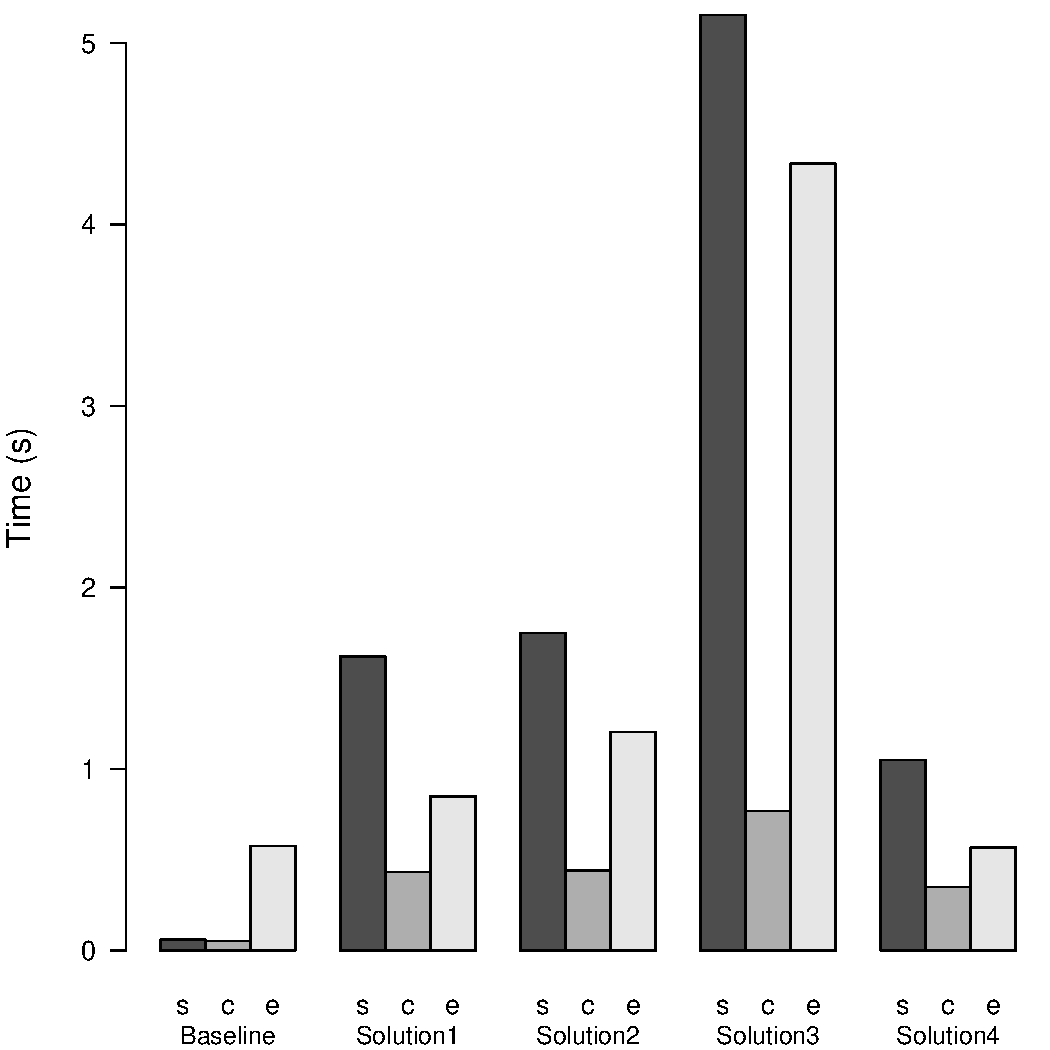
\includegraphics[width=\W]{figure/result/barplot-delete-rt.pdf} \label{fres:delete-}\label{fres:Delete-responsetime}}
		\subfigure[Throughput for Update operation]
		{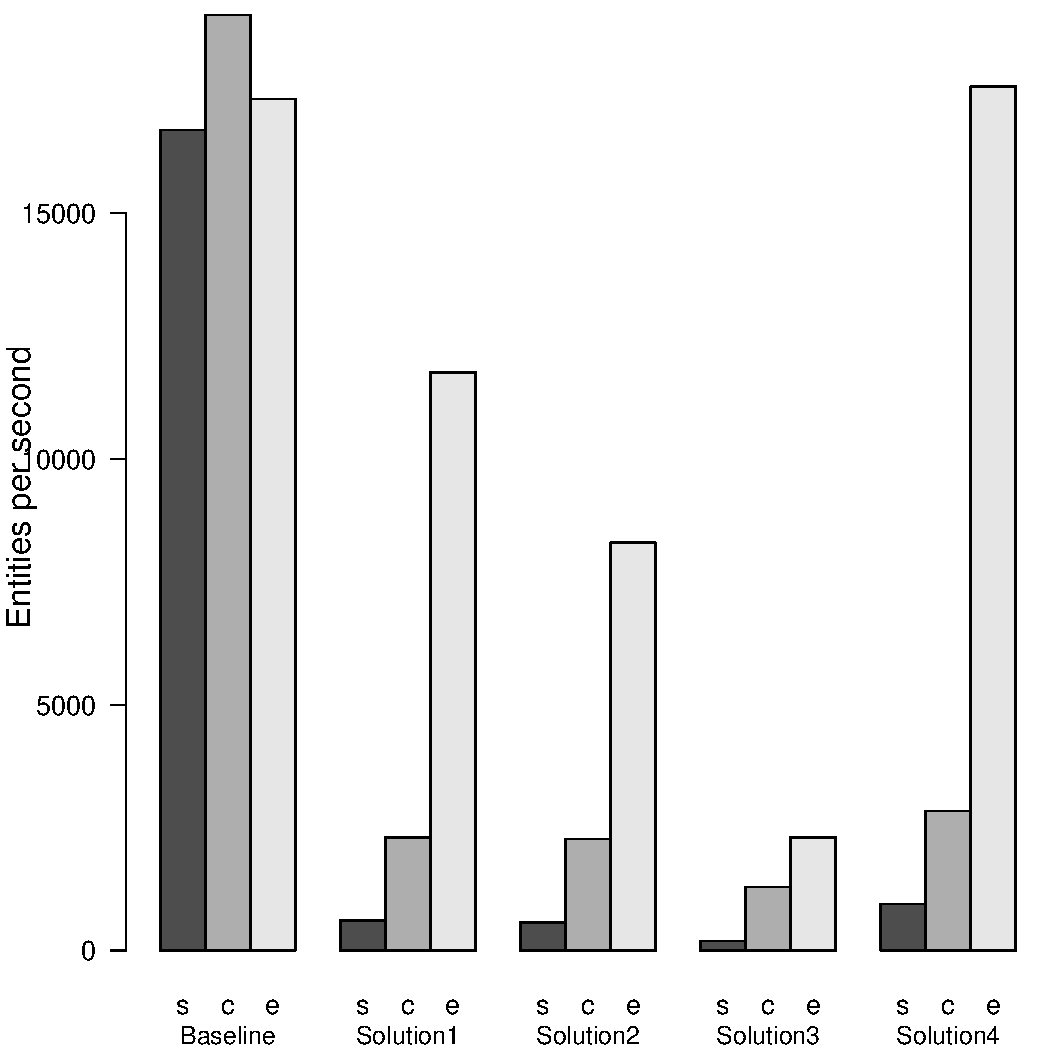
\includegraphics[width=\W]{figure/result/barplot-delete-tp.pdf} \label{fres:delete-}\label{fres:Delete-throughput}}
		\caption{Performance of Solutions in Update}\label{fres:Delete}
	\end{figure}
 
As seen in  the results, the \texttt{delete} in \texttt{Enrolment}
is the fastest in all the solutions, while  \texttt{delete} in
\texttt{Student} is the slowest. The \texttt{delete} operation on 
\texttt{Course} is faster than deleting \texttt{Student} entities but it
always takes more time than \texttt{delete} in \texttt{Enrolment}.

As seen in \texttt{update}, the difference in  performance of the operation
on the different entities is because of the referential integrity rules on
child and parent entities. Deleting \texttt{Enrolment} entities is faster as it 
does not invoke any referential integrity validations since \texttt{Enrolment}
has no child dependencies in it.
However, this operation is  slower than the baseline in all the solutions
because it involves accessing metadata to retrieve the relevant constraints of
\texttt{Enrolment} in order to determine if any child dependencies exist or
not.

Deleting \texttt{Student} entities is a cascaded operation which involves
deleting the child entities in the \texttt{Enrolment} column family. This
operation is slower because  the relevant constraints need to be  accessed and
the child entities in \texttt{Enrolment}  that have a reference to the
\texttt{Student} have to be deleted. 

Similarly, \texttt{delete} on \texttt{Course} entities also involves accessing
the relevant constraints and finding the child dependencies in
\texttt{Enrolment}. However, in the experiments,  all the entities in
\texttt{Enrolment} are already deleted before \texttt{delete} is invoked on
\texttt{Course} entities. Hence, \texttt{delete} in \texttt{Course} actually
deletes the entities as there are no existing child dependencies.
Notice that \texttt{delete} on \texttt{Course} involves the time to access
metadata as well as \texttt{Enrolment} in order to search for any existing child
dependencies and values are deleted from a single column family. However,
\texttt{delete} on \texttt{Student} entities involve deleting values from two
column families (\texttt{Student} and \texttt{Enrolment}). This
makes \texttt{delete} in \texttt{Course} faster than \texttt{delete} in
\texttt{Student}.

Finally, Figures~\ref{fres:delete-response-time}
and~\ref{fres:delete-throughput} show the average response time and throughput
of \texttt{delete} on all the entities. It can be seen from these results that
Solution~4 takes the least time to complete a \texttt{delete} operation on each
entity, while Solution~3 takes the most time. Since Solution~4 caches the
metadata of all the entities, it avoids multiple accesses to the
\texttt{Metadata} column family whereas Solution~3 requires accessing
\texttt{Metadata} each time a constraint has to be accessed for an entity. The
performance of Solutions~1 and 2 are comparable to each other even though
Solution~2 takes slightly more time due to its additional search operation to
locate the top row.

When compared to the baseline, all the solutions take longer to delete entities.
As mentioned previously, this is because all the solutions involve accessing
relevant constraints and performing validations.
Solutions~1 and 2 are almost 2 times slower than baseline  when
\texttt{Enrolment} entities are deleted while Solution~3 is almost 7 times
slower. Solution~4 is almost similar to the baseline in this case  which shows
that accessing the metadata does not cause much difference in the performance.


However, in a cascaded delete which includes referential integrity validations
Solutions~1 and 2 are more than 23 times slower than the
baseline while Solution~3 is almost 80
times slower. Solution~4  is up to 17 times slower than the baseline.



\begin{landscape}
		\begin{figure}
		\centering
		\newcommand{\W}{.4\textwidth}
			\subfigure[Delete on Student]
			{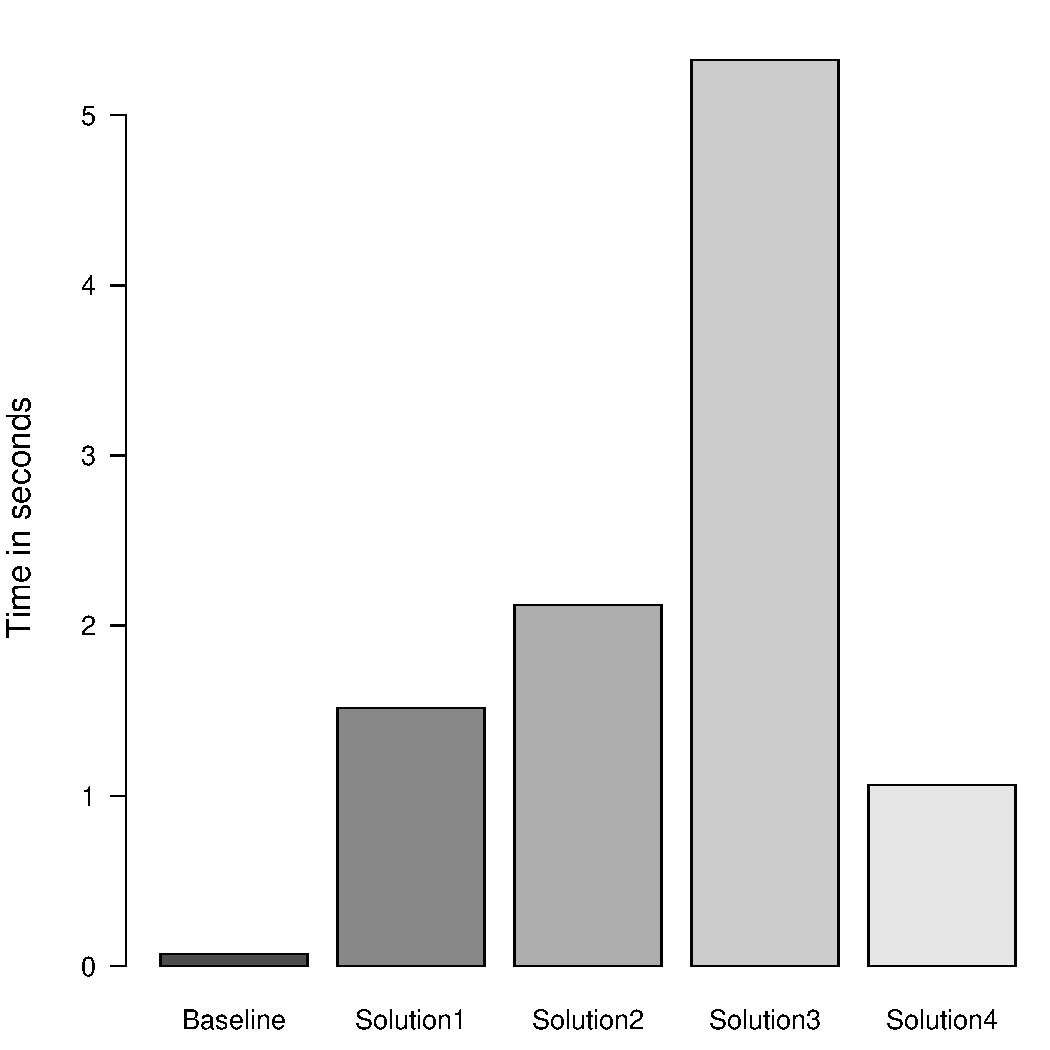
\includegraphics[width=\W]{figure/result/barplot-delete_student-rt.pdf}
			\label{fres:delete-user}}
			\subfigure[Delete on Course]
			{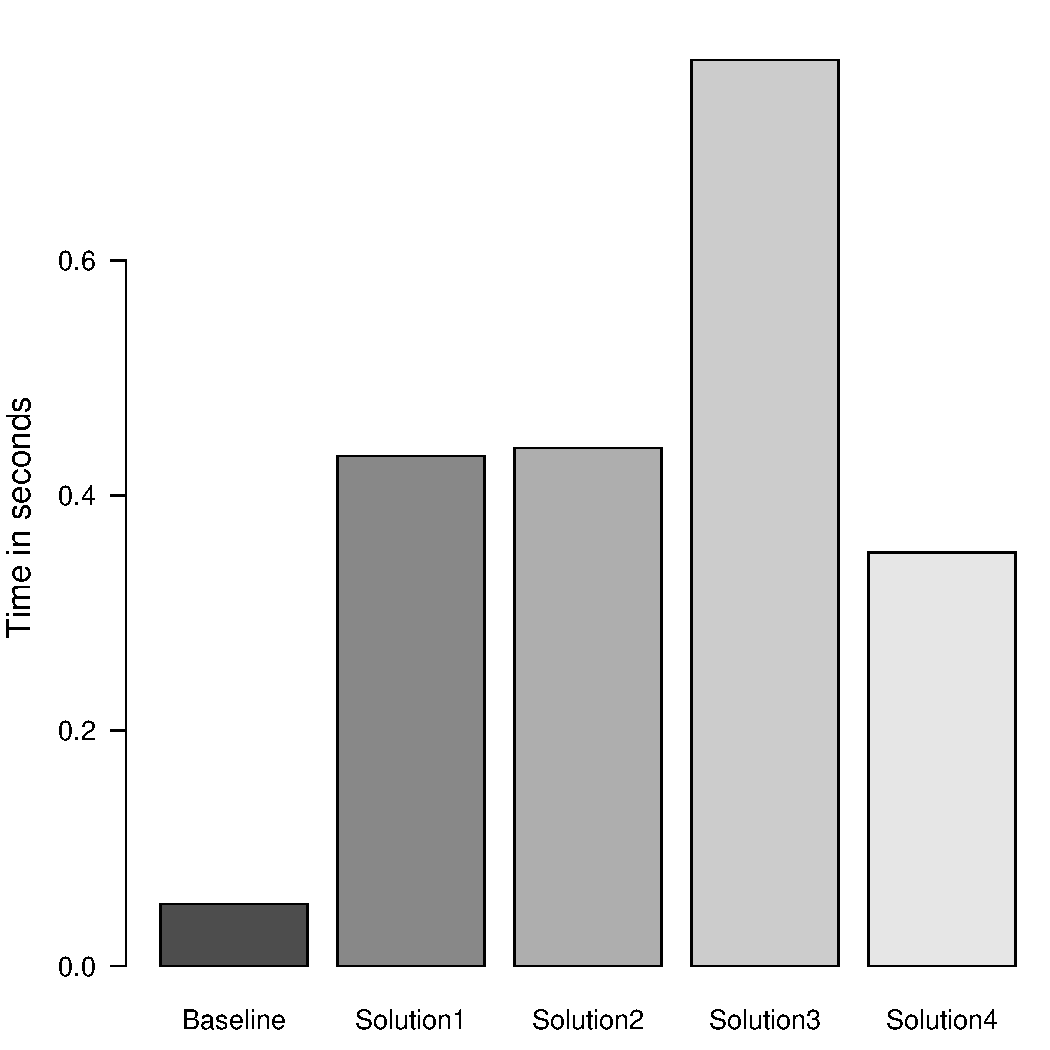
\includegraphics[width=\W]{figure/result/barplot-delete_course-rt.pdf}
			\label{fres:delete-course}}
			\subfigure[ Delete on Enrolment ]
			{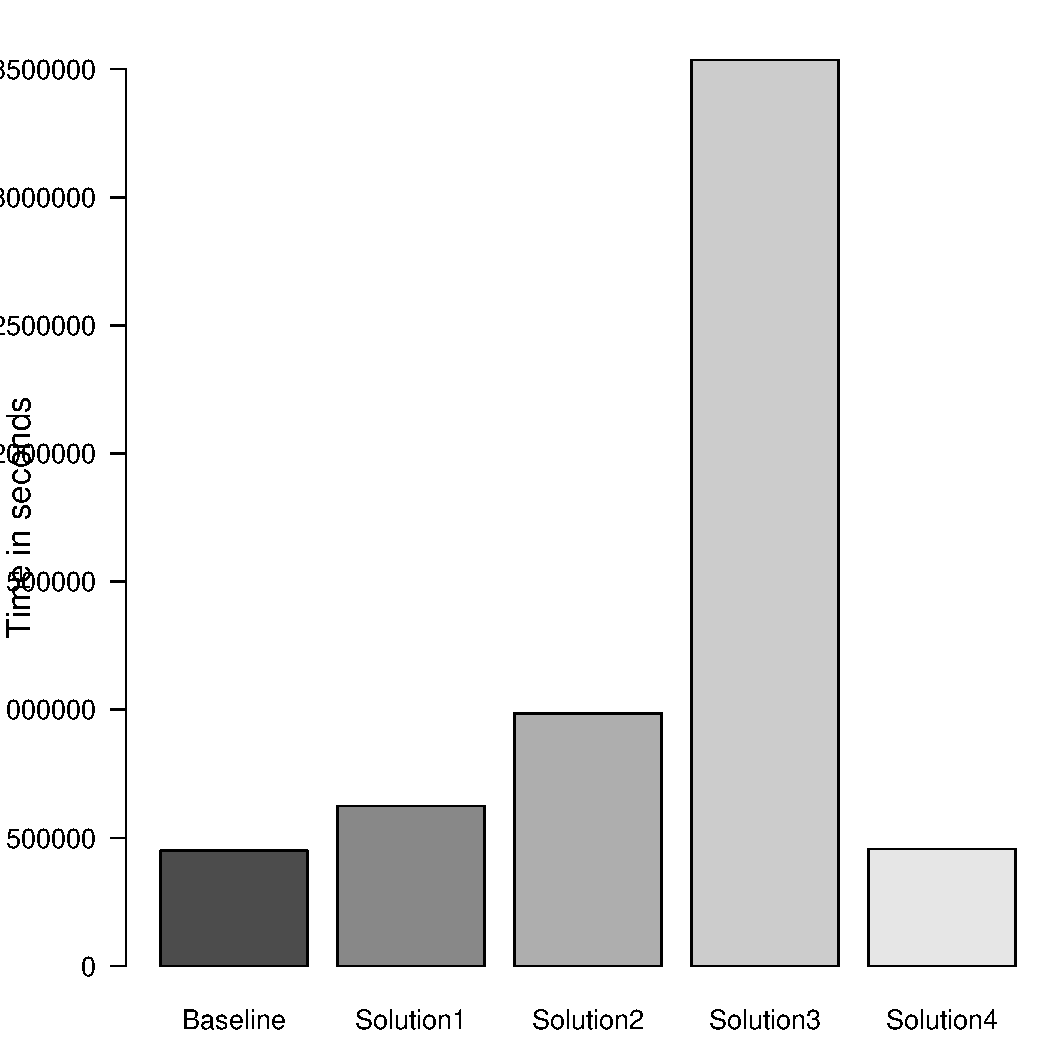
\includegraphics[width=\W]{figure/result/barplot-delete_enrolment-rt.pdf}
			\label{fres:delete-enrolment}}
			\caption{Response time deleting entities}\label{fres:delete-response-time}
						
			\subfigure[Delete on Student]
			{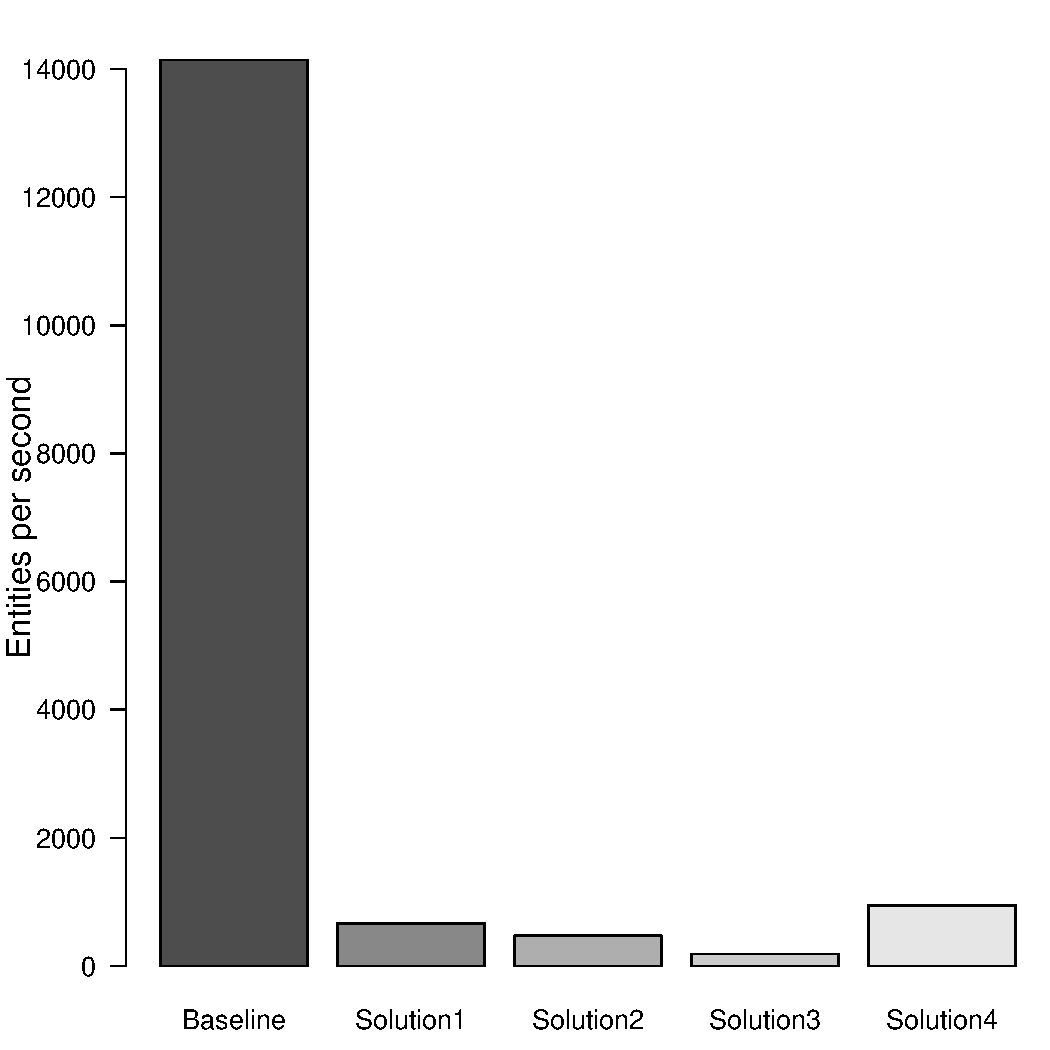
\includegraphics[width=\W]{figure/result/barplot-delete_student-tp.pdf} \label{fres:delete-}}
			\subfigure[Delete on Course]
			{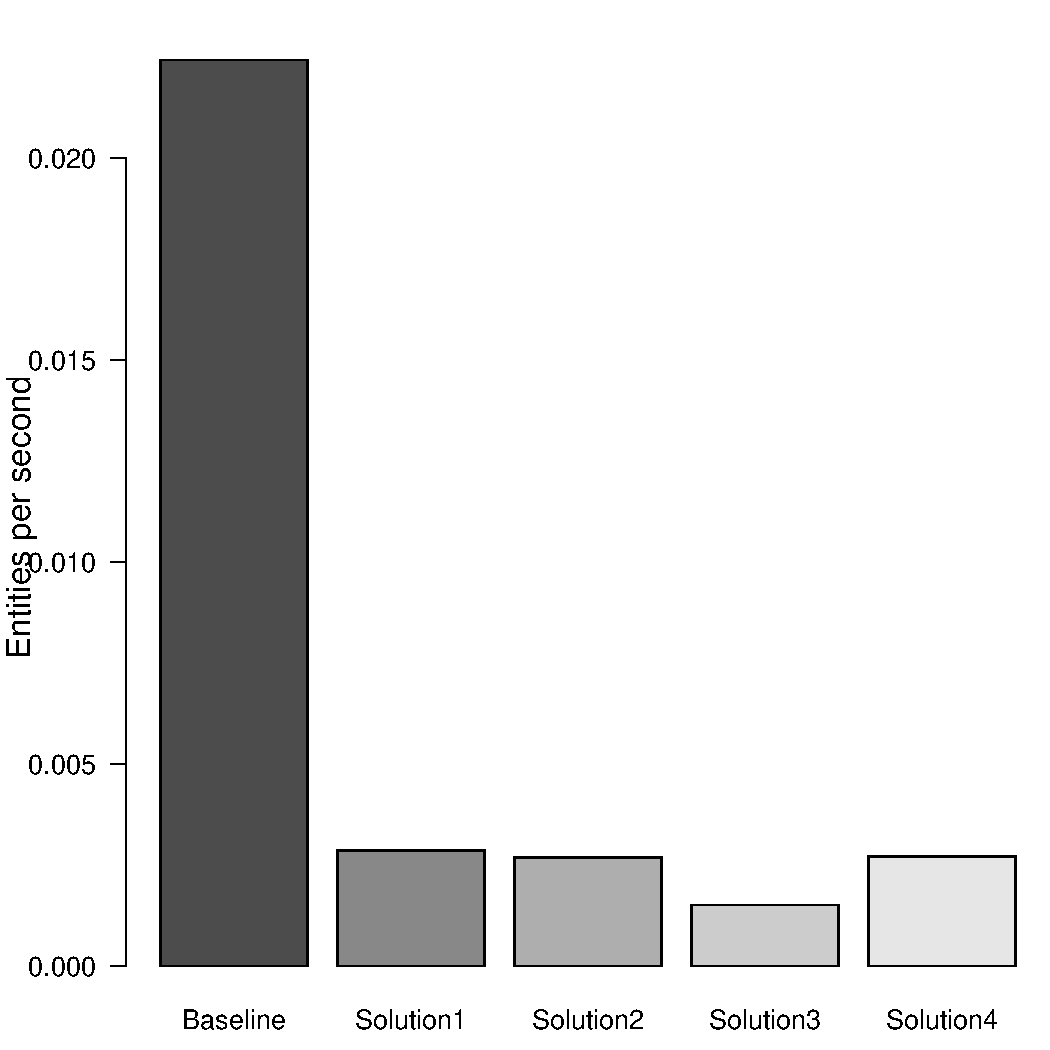
\includegraphics[width=\W]{figure/result/barplot-delete_course-tp.pdf} \label{fres:delete-}}
			\subfigure[Delete on Enrolment]
			{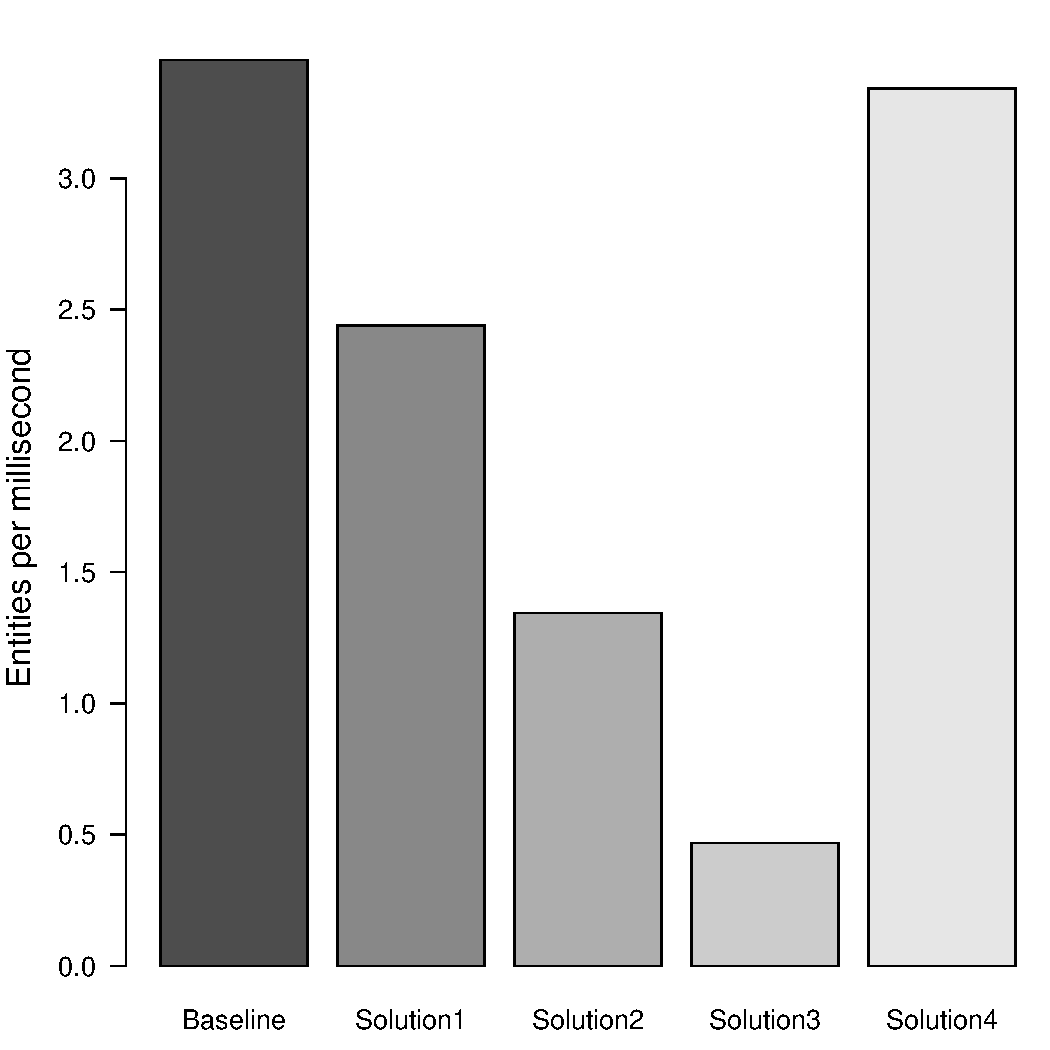
\includegraphics[width=\W]{figure/result/barplot-delete_enrolment-tp.pdf} \label{fres:delete-}}
			\caption{Throughput deleting entities}\label{fres:delete-throughput}
		\end{figure}
\end{landscape}
